The change we will make is to the structure of the partition shift preconditioner is replacing the diagonal of the matrix from the identity to inverse of the diagonal of the matrix it is applied to. Meaning combining Jacobi preconditioning and our partition shift preconditioner to get a new preconditioner we will call Shifted Jacobi preconditioner. This means our new preconditioner consistent of system specific part, the main diagonal, and a general learned part, the partitioned superdiagonal. A constraint that the new preconditioner has for the matrix it is applied to is that all diagonal entries of the matrix has to have a nonzero value. 

To test this new preconditioner we will run the learning algorithm with the same parameters as the previous test in section \ref{sec: Improve func} table \ref{table: improvement func test config}, with the only change being the preconditioner.

\begin{table}[H]
    \center
    \begin{tabular}{|l|r|r|r|}
        \hline
        Seed &SIGN& MEDIAN & MEAN  \\\hline
        0 & 39 & 25 & 29 \\
        1 & 37 & 27 & 23 \\
        2 & 58 & 27 & 26 \\
        3 & 65 & 37 & 34 \\\hline
    \end{tabular}
    \caption{Number of times a new preconditioner was accept. A row for each seed and column for each improvement function.}
    \label{table: Jacobi par shift improvement count}
\end{table}

\begin{figure}[H]
    \center
    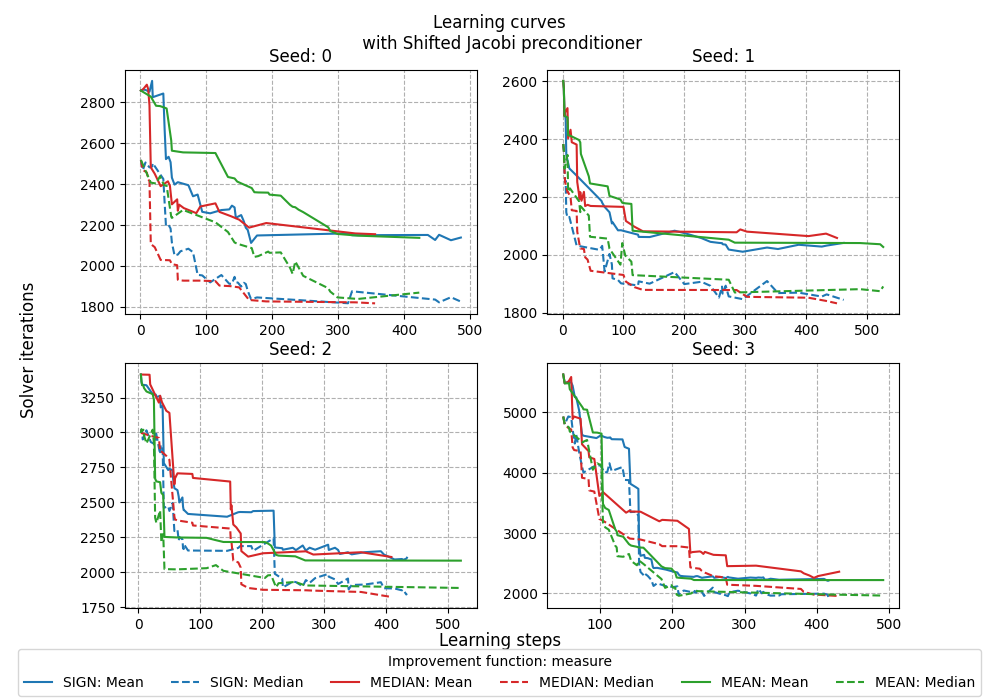
\includegraphics[width=1\textwidth]{plots/jacobi_par_shift_learning_curve.png}
    \caption{Learning curves for testing Shifted Jacobi preconditioner. The plot has the same structure as figure \ref{fig: initial improv learn curve}, a plot for each seed, colours indicate improvement function, and line style corresponds to solver iteration count mean or median.}
    \label{fig: Jacobi par shift learning curves}
\end{figure}


From the learning curves in figure \ref{fig: Jacobi par shift learning curves}, we can see clear improvements when comparing to the learning curves from the previous tests in figure \ref{fig: initial improv learn curve}. The mean and median solver iteration count decrease significant amount during the learning for all three improvement function, where as before with MEDIAN improvement function had difficulty finding improvements to the preconditioner. Even when the initial preconditioner starts with mean solver iteration count above 5000 for seed 3 and the final iteration counts is only a bit higher compared to the other seeds, but this may be because the data set and not the preconditioner. 

Another improvement is the number of accepted coefficient changes made during learning is considerably larger for MEAN and MEDIAN improvement functions and similar for SIGN, table \ref{table: Jacobi par shift improvement count}, again comparing to the previous learning tests in section \ref{sec: initial par shift}. This means that even before looking at the evaluation, we can expect the learned preconditioners being good. And lastly a new problem has occurred from the learning curves is that it looks like the learning has plateaued, example for seed 1 the amount of change that happens to the mean and median solver iteration count after learning step 150 is minimal compared to the earlier leaning step. This could mean that it has found the best preconditioner, that it has found a local minimum and the changes made to the preconditioner are not big enough to find a better minimum, or that it did not have enough steps iteration and not plateaued.

In the evaluations of the preconditioner on the test data, there is only a marginal improvement compared to Jacobi preconditioning on its own for the mean and median solver iteration counts, figure \ref{fig: jacobi par shift test measure}, and only with SIGN and MEAN improvement functions we get more than half of the systems having a lower solver iteration count than when using Jacobi preconditioning, figure \ref{fig: Jacobi par shift BvJ}. For the differences in improvement function there is very little difference in the evaluations of the learned preconditioners, with SIGN being slightly better across all the seeds for this reason and because it worked the best in the previous test we will only use the SIGN improvement function for all further testing of the learning algorithm and structural changes to the preconditioner. From this it is easy to say that these learned preconditioners with Jacobi diagonal are better than the previous learned preconditioners with identity diagonal, but only slightly better than the simple Jacobi preconditioning.


\begin{figure}[H]
    \center
    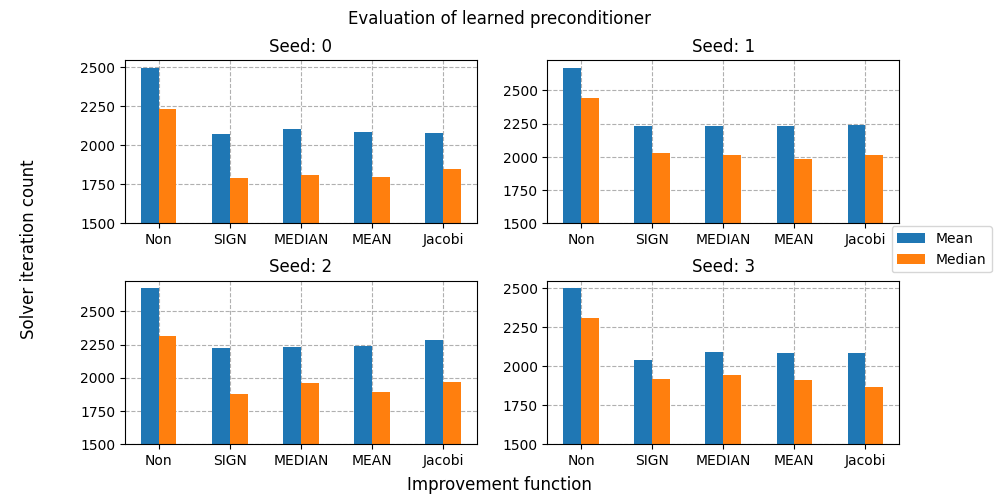
\includegraphics[width=1\textwidth]{plots/jacobi_par_shift_test_measure.png}
    \caption{Evaluation of the learned preconditioners with the same structure as figure \ref{fig: initial improv test measure with jacobi}. A plot for each seed, with a bars for the three improvement functions and 2 to compare with unpreconditioned and Jacobi preconditioned solver iteration count. Bar colours indicate mean (blue) and median (orange) solver iteration count.}
    \label{fig: jacobi par shift test measure}
\end{figure}

\begin{figure}[H]
    \center
    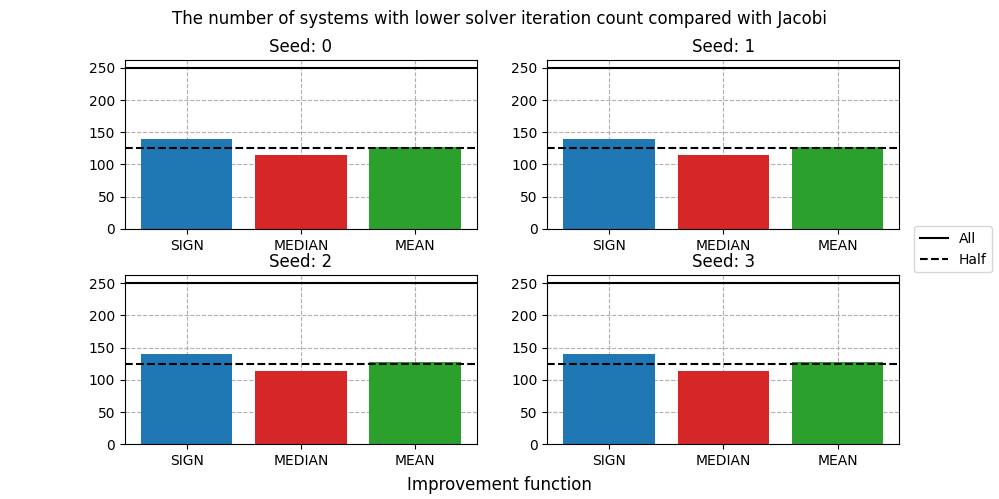
\includegraphics[width=0.95\textwidth]{plots/jacobi_par_shift_BvJ.png}
    \caption{Individual system comparison plot with the same structure as \ref{fig: initial improv BvJ}. A plot for each seed, bars for each improvement function, and lines to indicate all or half the systems.}
    \label{fig: Jacobi par shift BvJ}
\end{figure}

